\documentclass[a4paper,12pt]{article}
\usepackage{outline}
\usepackage{pmgraph}
\usepackage[normalem]{ulem}
\usepackage{comment} % enables the use of multi-line comments (\ifx \fi)
\usepackage{lipsum} %This package just generates Lorem Ipsum filler text.
\usepackage{fullpage} % changes the margin
\usepackage{listings}
\usepackage{color}
\usepackage{mdframed}
\usepackage{listings}
\usepackage{graphicx}
\graphicspath{ {../ScreenShots/} }
\renewcommand{\lstlistingname}{Code Block}% Listing -> Algorithm
\renewcommand{\lstlistlistingname}{List of \lstlistingname s}% List of Listings -> List of Algorithms

\linespread{1.5}
%--------------------Indention
\setlength{\parindent}{15pt}
\lstset{frame=shadowbox, rulesepcolor=\color{white}}
\mdfsetup{frametitlealignment=\center}
\lstset{
  numbers=left,
  stepnumber=1,
  firstnumber=1,
  numberfirstline=true
}

\begin{document}
\section*{Objective}

\hspace{15pt}In the last lab, two different methods to create digital circuits in Verilog was introduced. One was
structural method and the other was dataflow modeling. In this lab, a $3^{rd}$ method will be used, behavioral modeling.

This lab consisted of three separate experiments. For \textbf{Experiment 1}, the multiplexers created last lab will
be converted into behavioral Verilog. In \textbf{Experiment 2}, students will describe, using behavioral Verilog, binary encoders and decoders. Finally, \textbf{Experiment 3} will introduce logic synthesis, as well as translating HDL code into implementable digital logic. The code written in Experiment 2 will be synthesized and programed onto a Spartan 3E in order to further verify that the encoder and decoder described is in fact correct.

\section*{Design}

\textbf{Experiment 1}
% Verilog code template
 \lstinputlisting[language=Verilog,,caption=4-Bit ALU ]{../Code/four_bit_mux_behavioral.v}

\hspace{-15pt}\textbf{Experiment 2}

\hspace{-15pt}\textbf{Experiment 3}

\section*{Results}

\textbf{Experiment 1}

% \begin{figure}[h]
%   \begin{center}
%     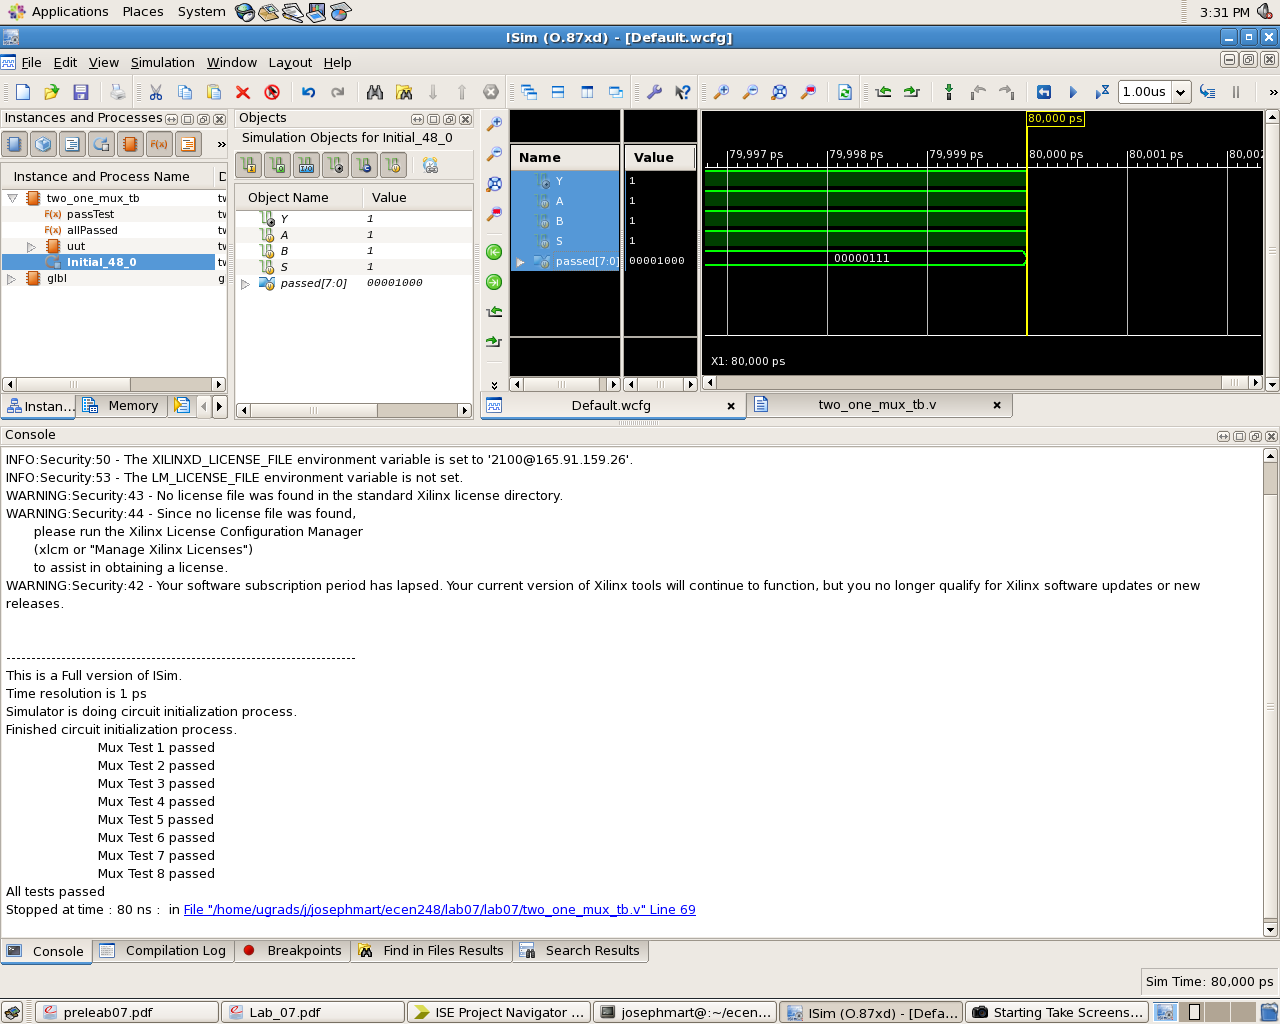
\includegraphics[scale=0.1]{1_1_1.png}
%     \caption{\textit{2-Bit 2:1 MUX Plots}}
%   \end{center}
% \end{figure}
%
% \begin{figure}[h]
%   \begin{center}
%     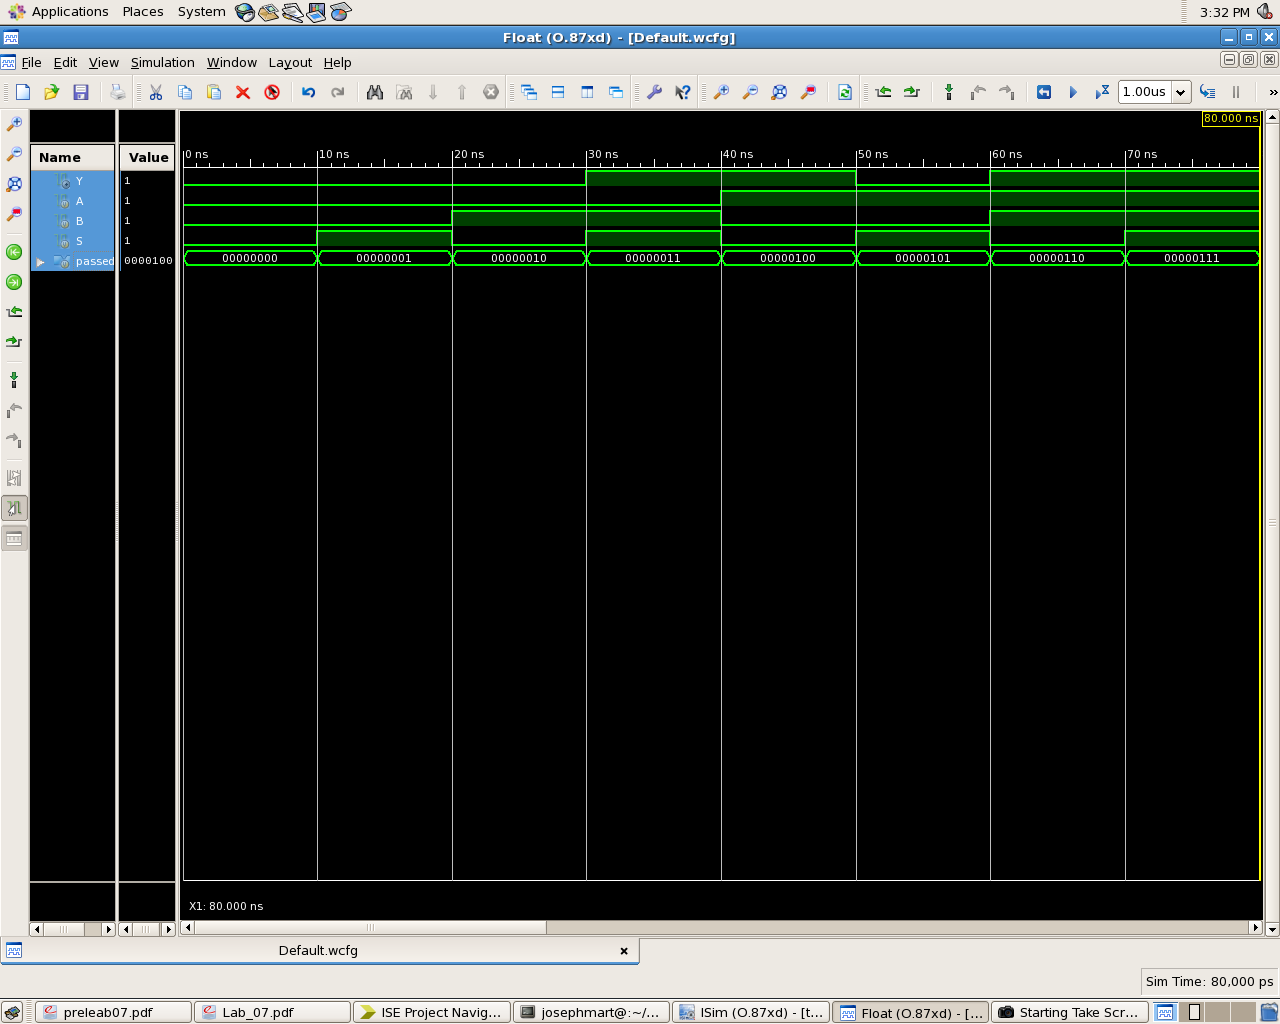
\includegraphics[scale=0.1]{1_1_2.png}
%     \caption{\textit{2-Bit 2:1 MUX Plots}}
%   \end{center}
% \end{figure}
%
% \begin{figure}[h]
%   \begin{center}
%     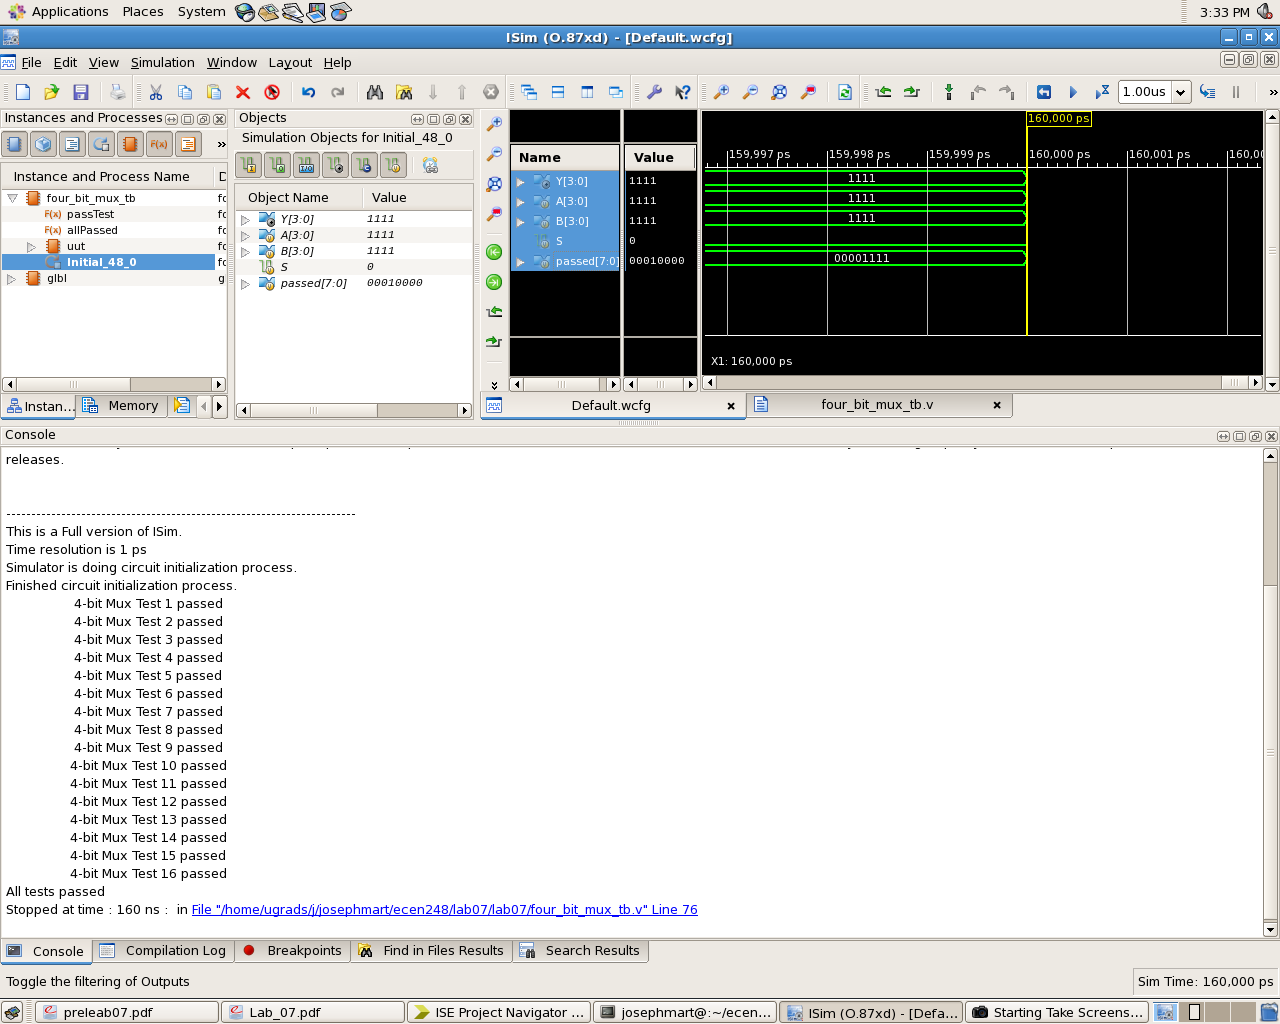
\includegraphics[scale=0.1]{1_2_1.png}
%     \caption{\textit{2-Bit 2:1 MUX Plots}}
%   \end{center}
% \end{figure}
%
% \begin{figure}[h]
%   \begin{center}
%     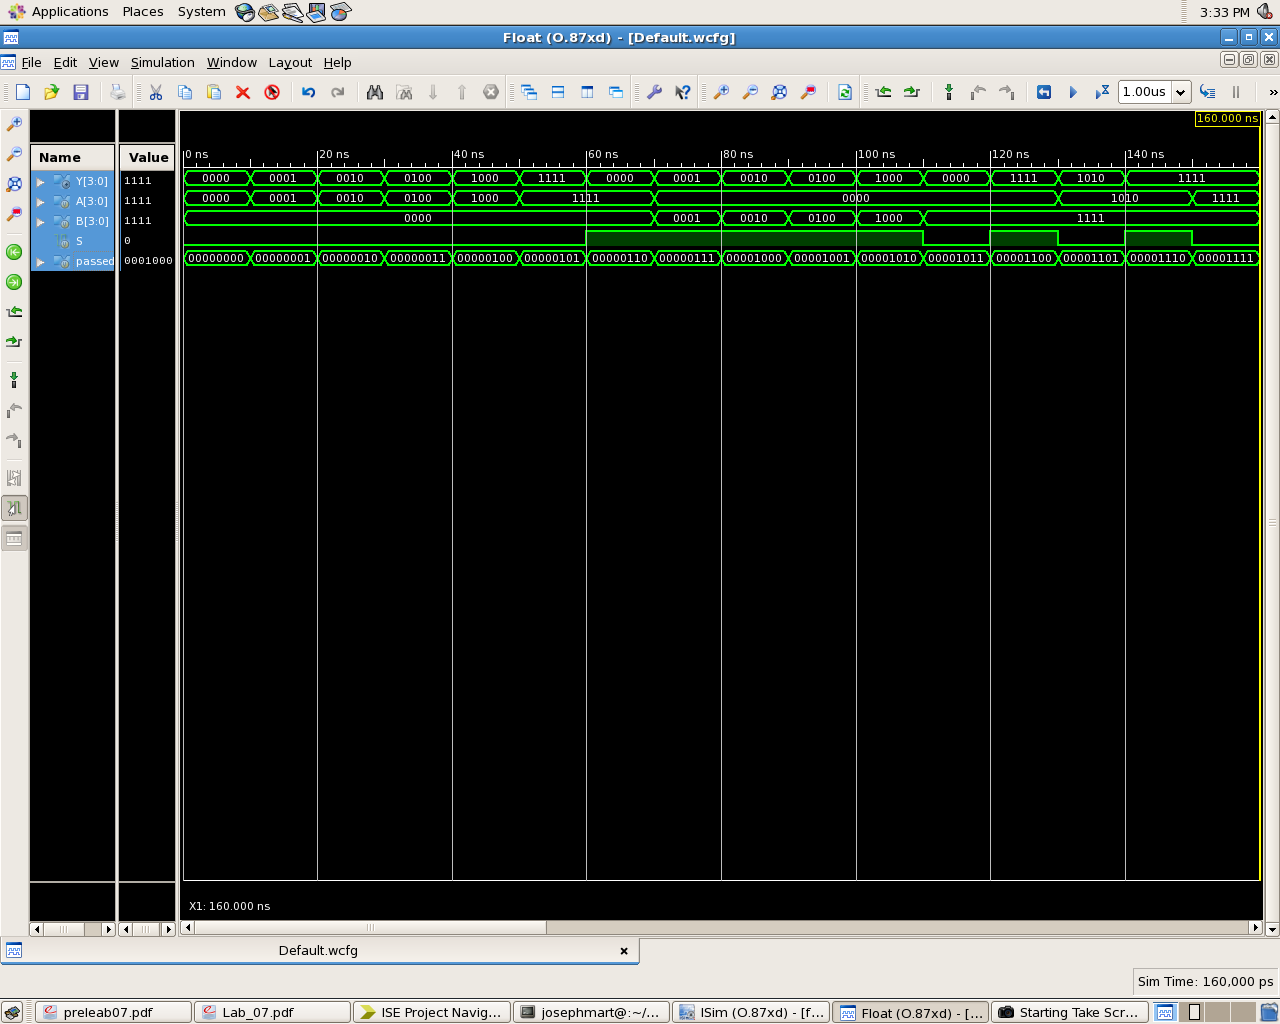
\includegraphics[scale=0.1]{1_2_2.png}
%     \caption{\textit{2-Bit 2:1 MUX Plots}}
%   \end{center}
% \end{figure}
%
% \begin{figure}[h]
%   \begin{center}
%     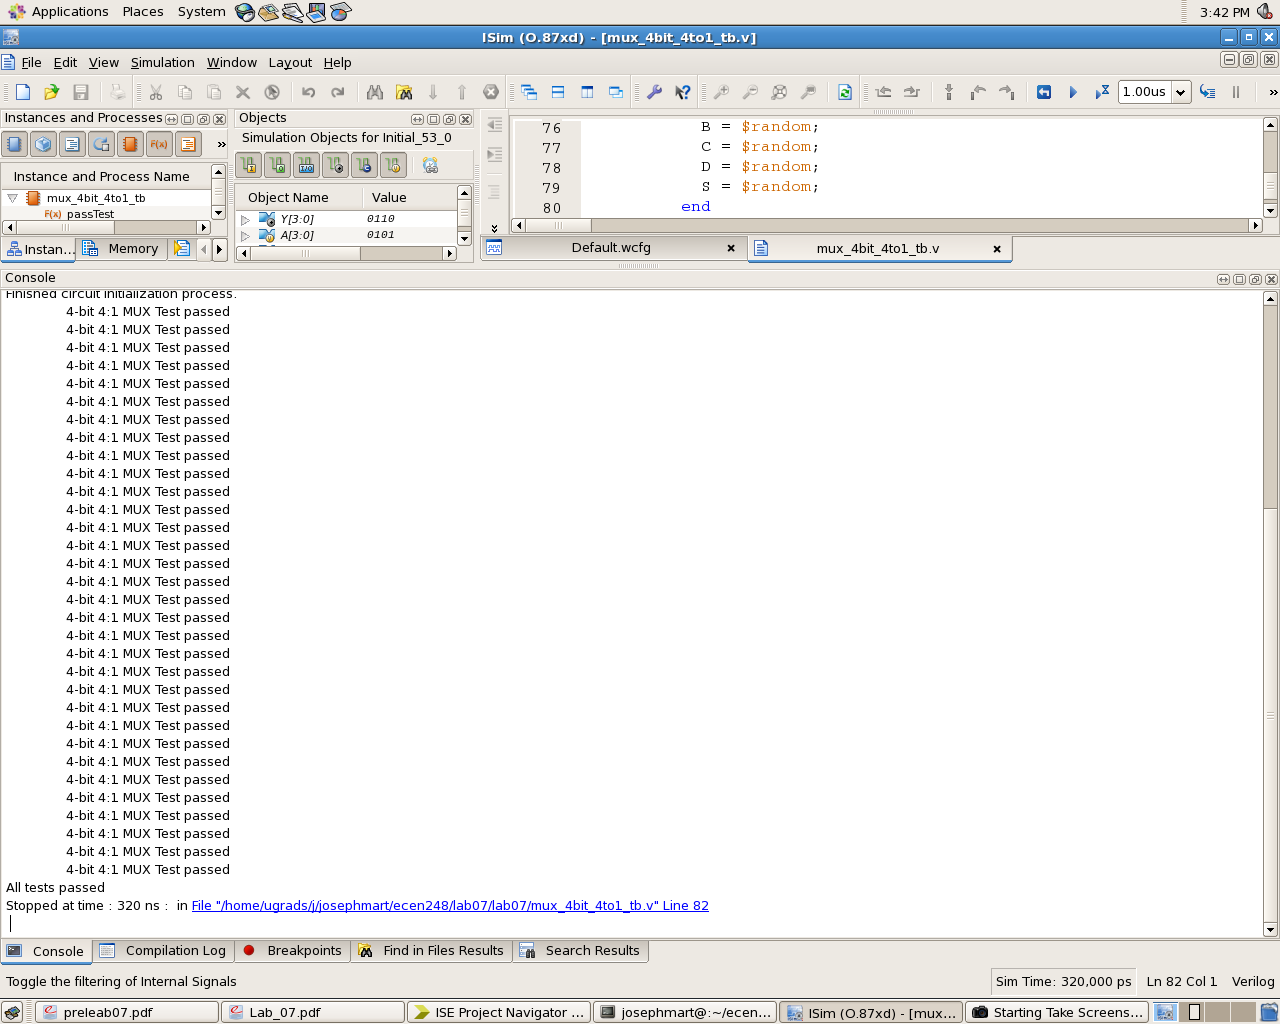
\includegraphics[scale=0.1]{1_3_1.png}
%     \caption{\textit{2-Bit 2:1 MUX Plots}}
%   \end{center}
% \end{figure}
%
% \begin{figure}[h]
%   \begin{center}
%     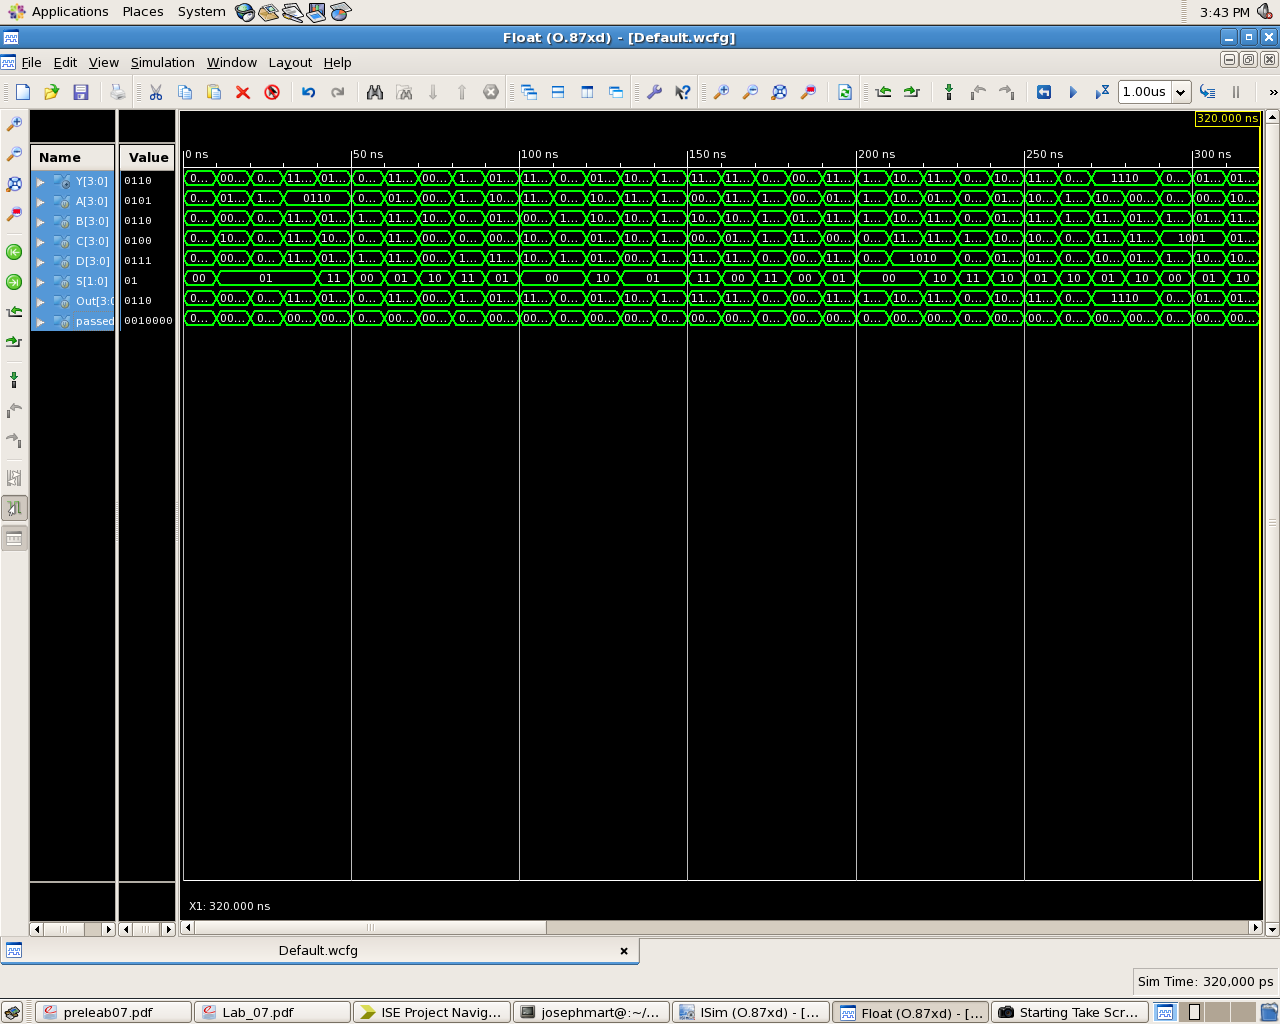
\includegraphics[scale=0.1]{1_3_2.png}
%     \caption{\textit{2-Bit 2:1 MUX Plots}}
%   \end{center}
% \end{figure}
%
% \hspace{-15pt}\textbf{Experiment 2}
%
% \begin{figure}[h]
%   \begin{center}
%     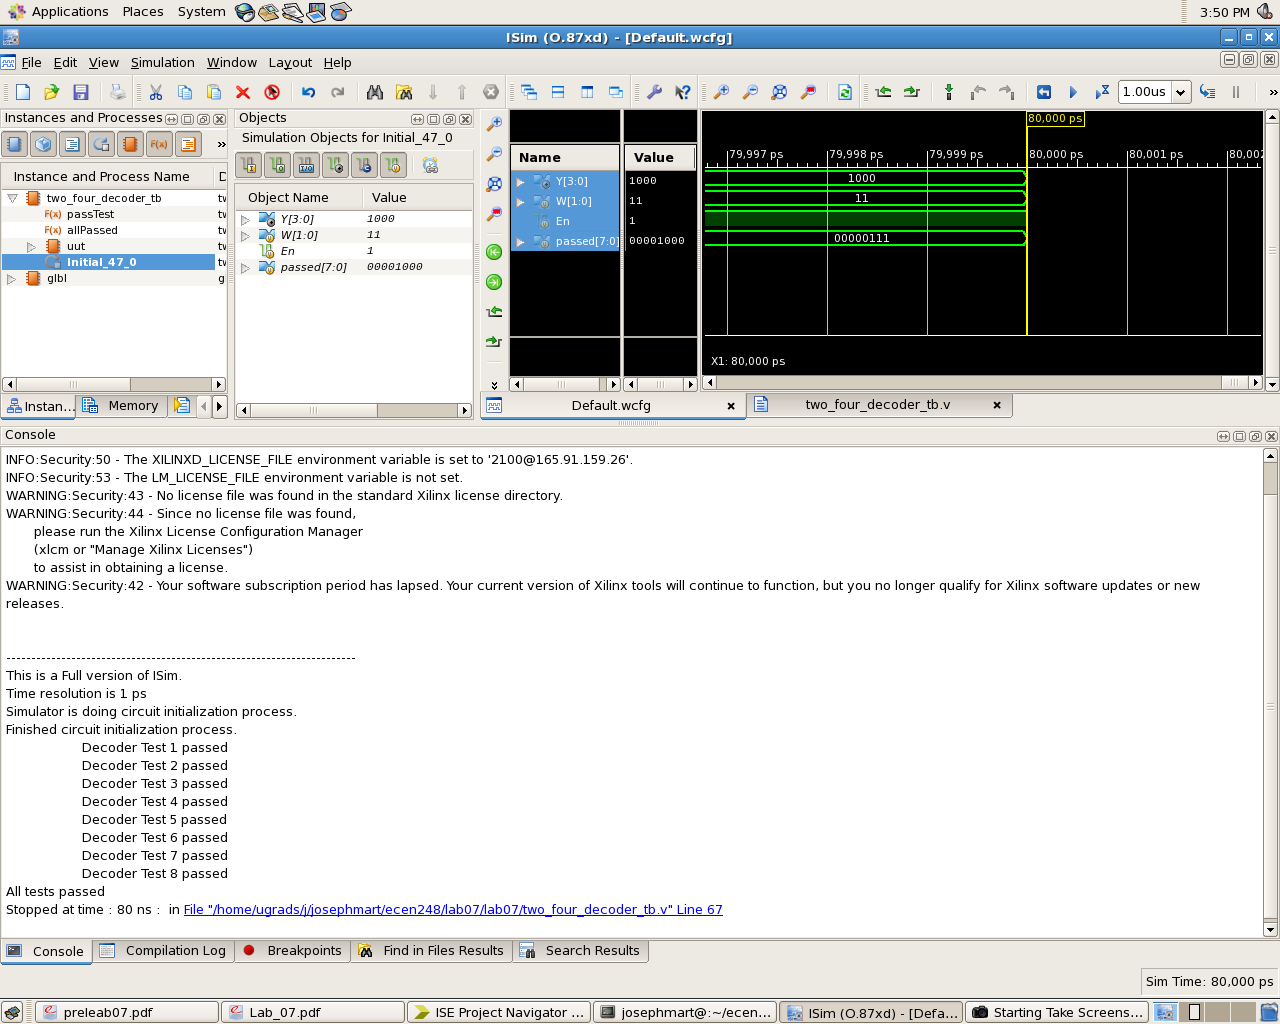
\includegraphics[scale=0.1]{2_1_1.png}
%     \caption{\textit{2-Bit 2:1 MUX Plots}}
%   \end{center}
% \end{figure}
%
% \begin{figure}[h]
%   \begin{center}
%     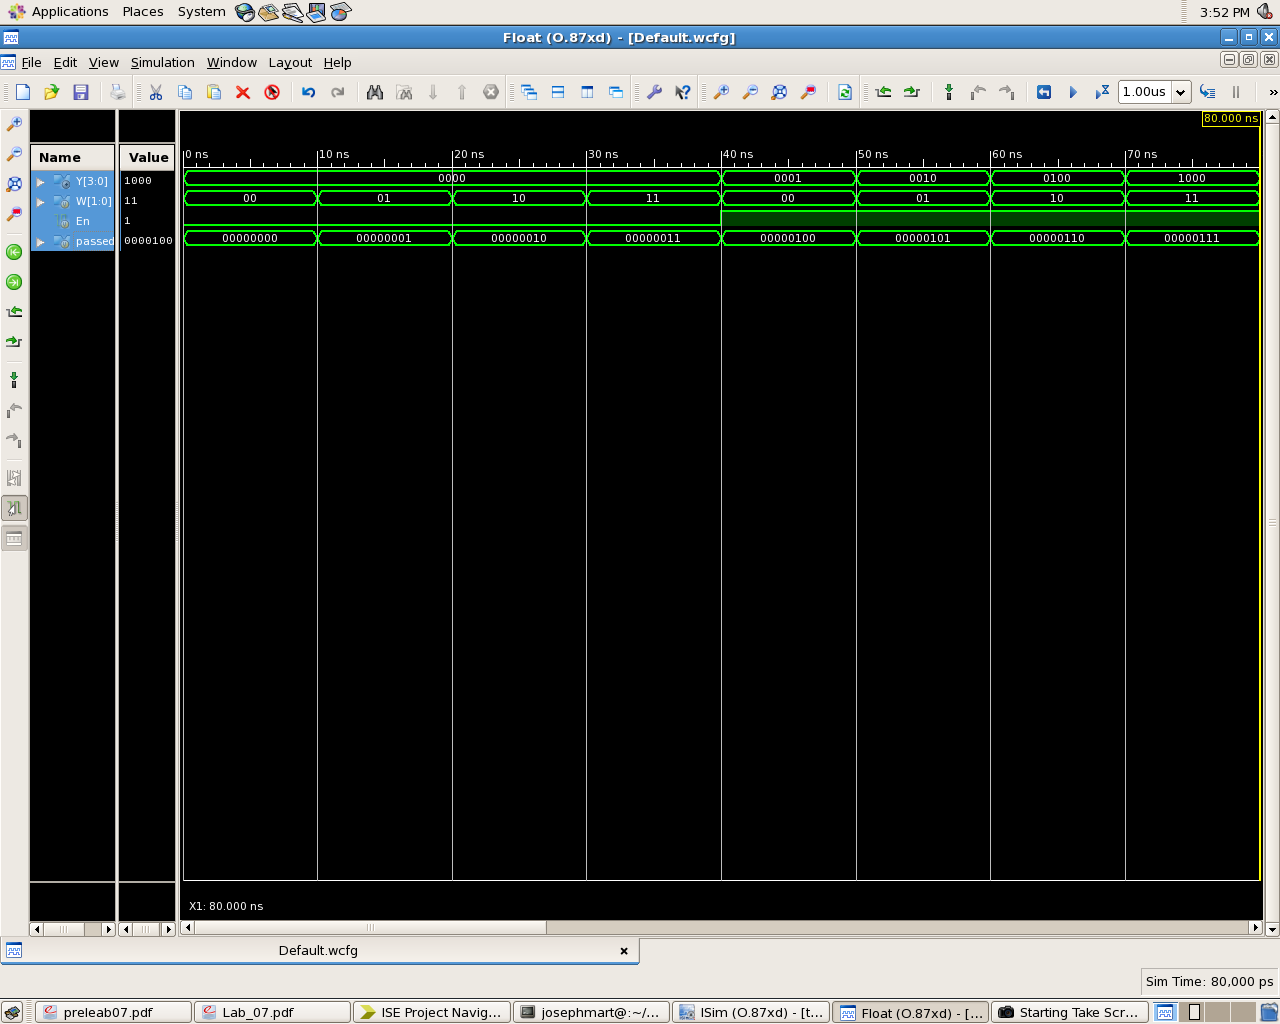
\includegraphics[scale=0.1]{2_1_2.png}
%     \caption{\textit{2-Bit 2:1 MUX Plots}}
%   \end{center}
% \end{figure}
%
% \begin{figure}[h]
%   \begin{center}
%     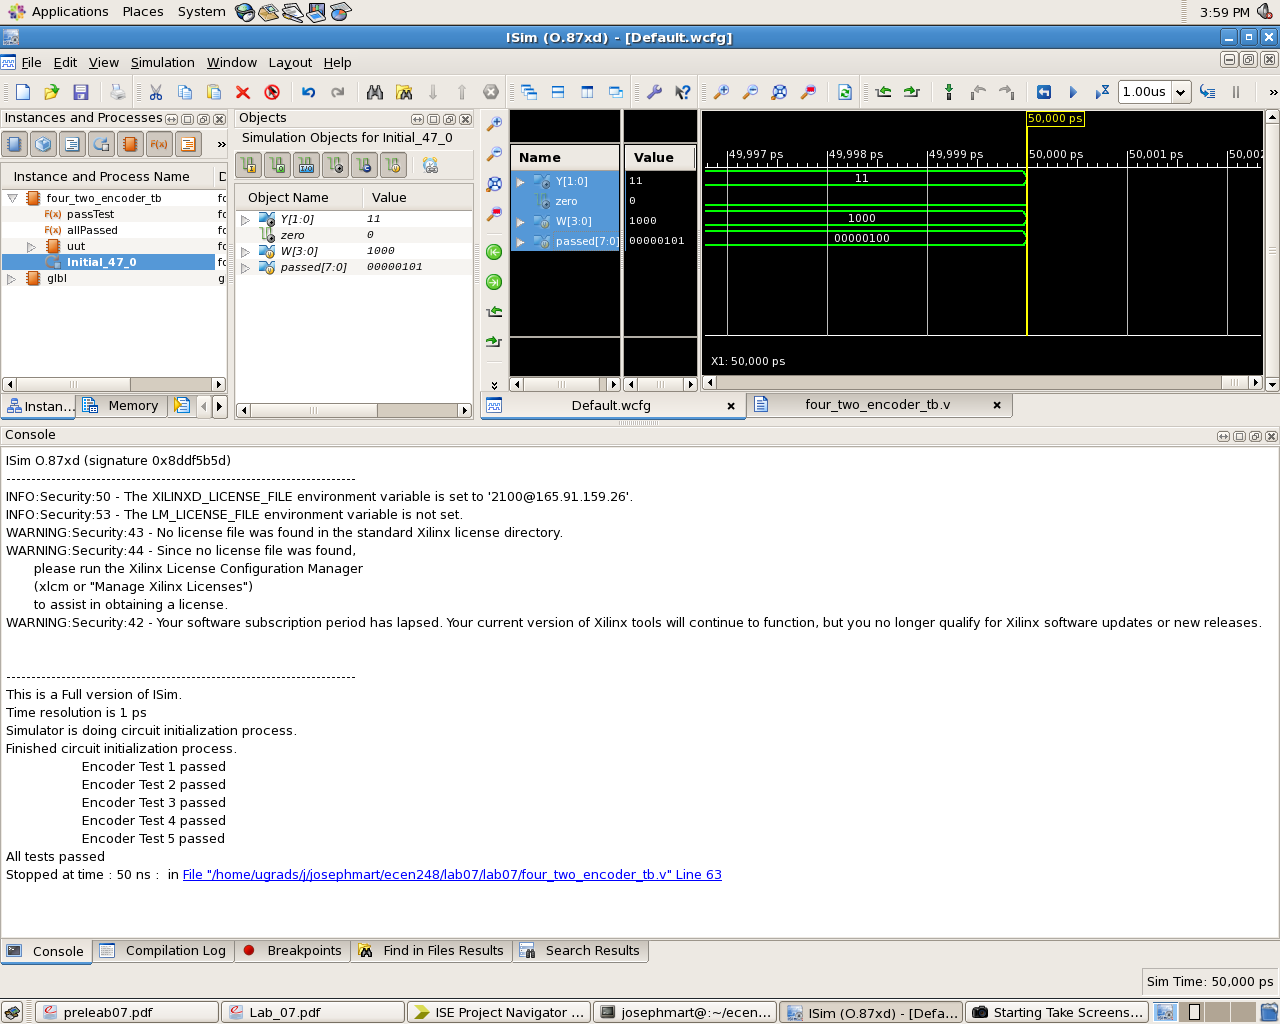
\includegraphics[scale=0.1]{2_2_1.png}
%     \caption{\textit{2-Bit 2:1 MUX Plots}}
%   \end{center}
% \end{figure}
%
% \begin{figure}[h]
%   \begin{center}
%     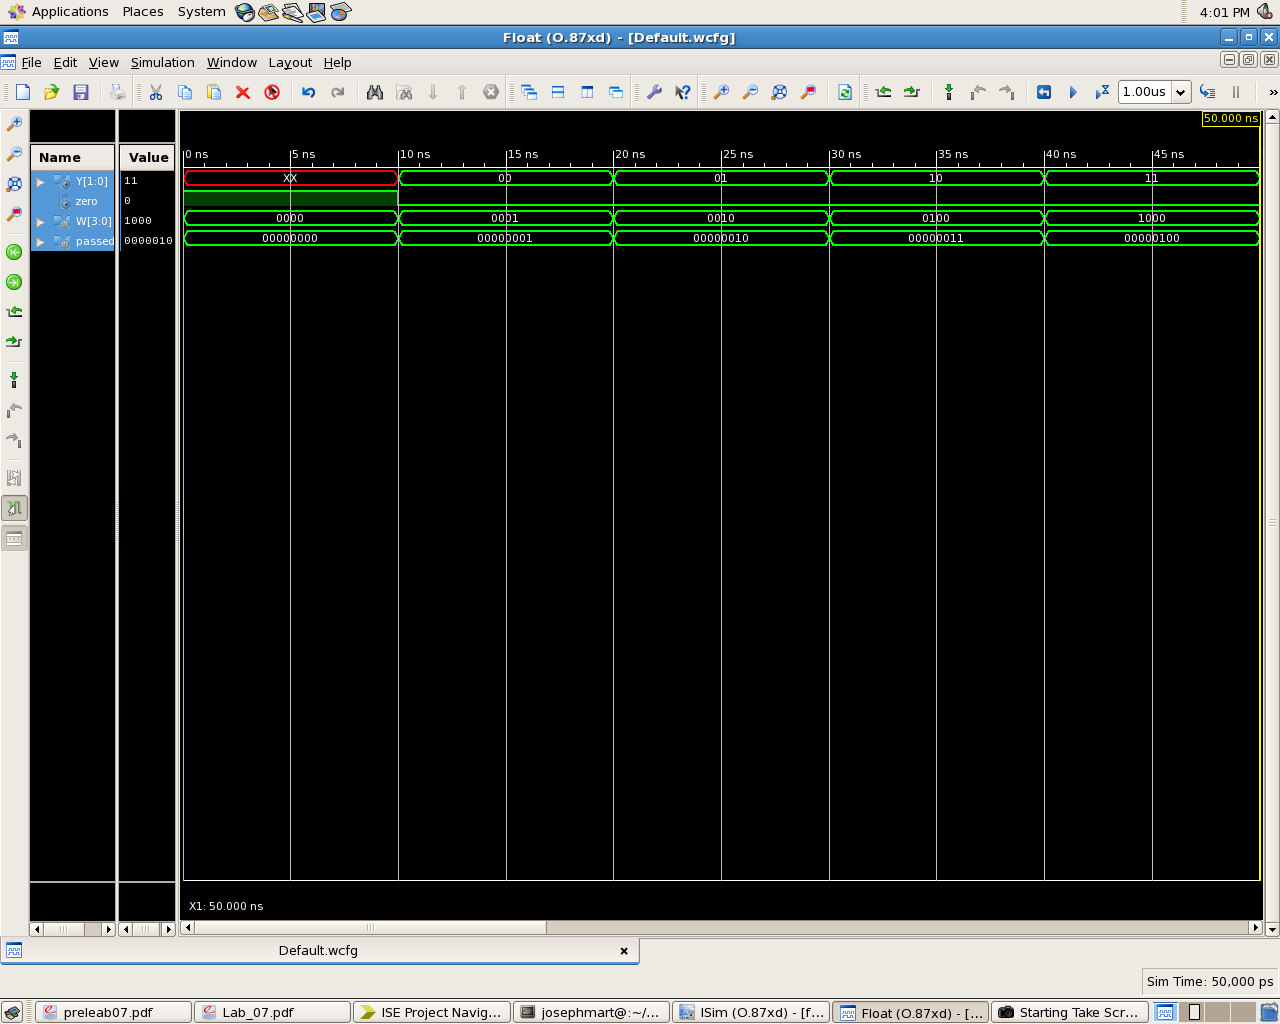
\includegraphics[scale=0.1]{2_2_2.png}
%     \caption{\textit{2-Bit 2:1 MUX Plots}}
%   \end{center}
% \end{figure}
%
% \begin{figure}[h]
%   \begin{center}
%     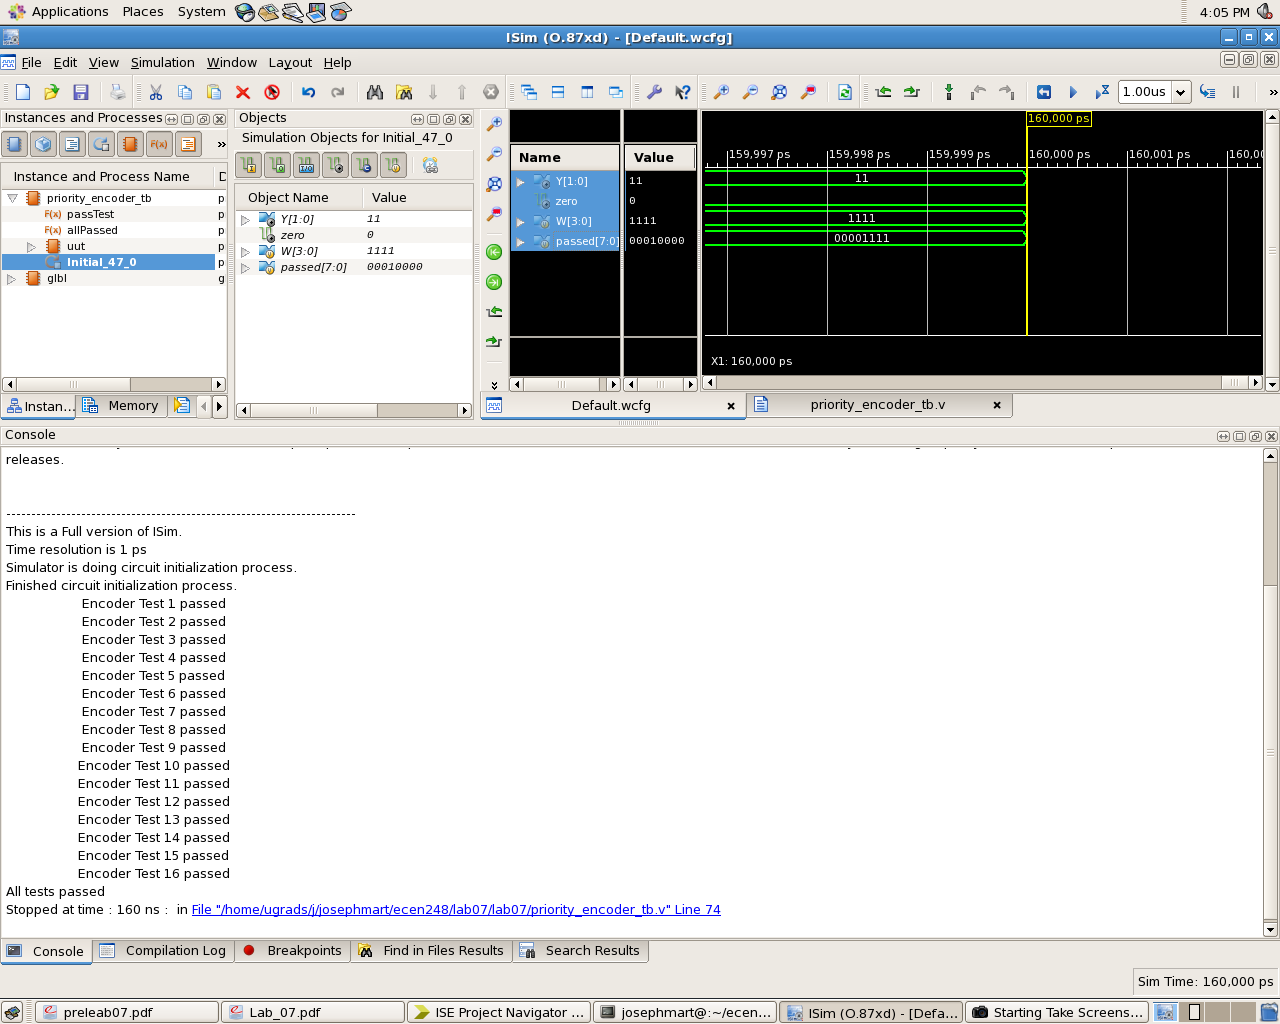
\includegraphics[scale=0.1]{2_3_1.png}
%     \caption{\textit{2-Bit 2:1 MUX Plots}}
%   \end{center}
% \end{figure}
%
% \begin{figure}[h]
%   \begin{center}
%     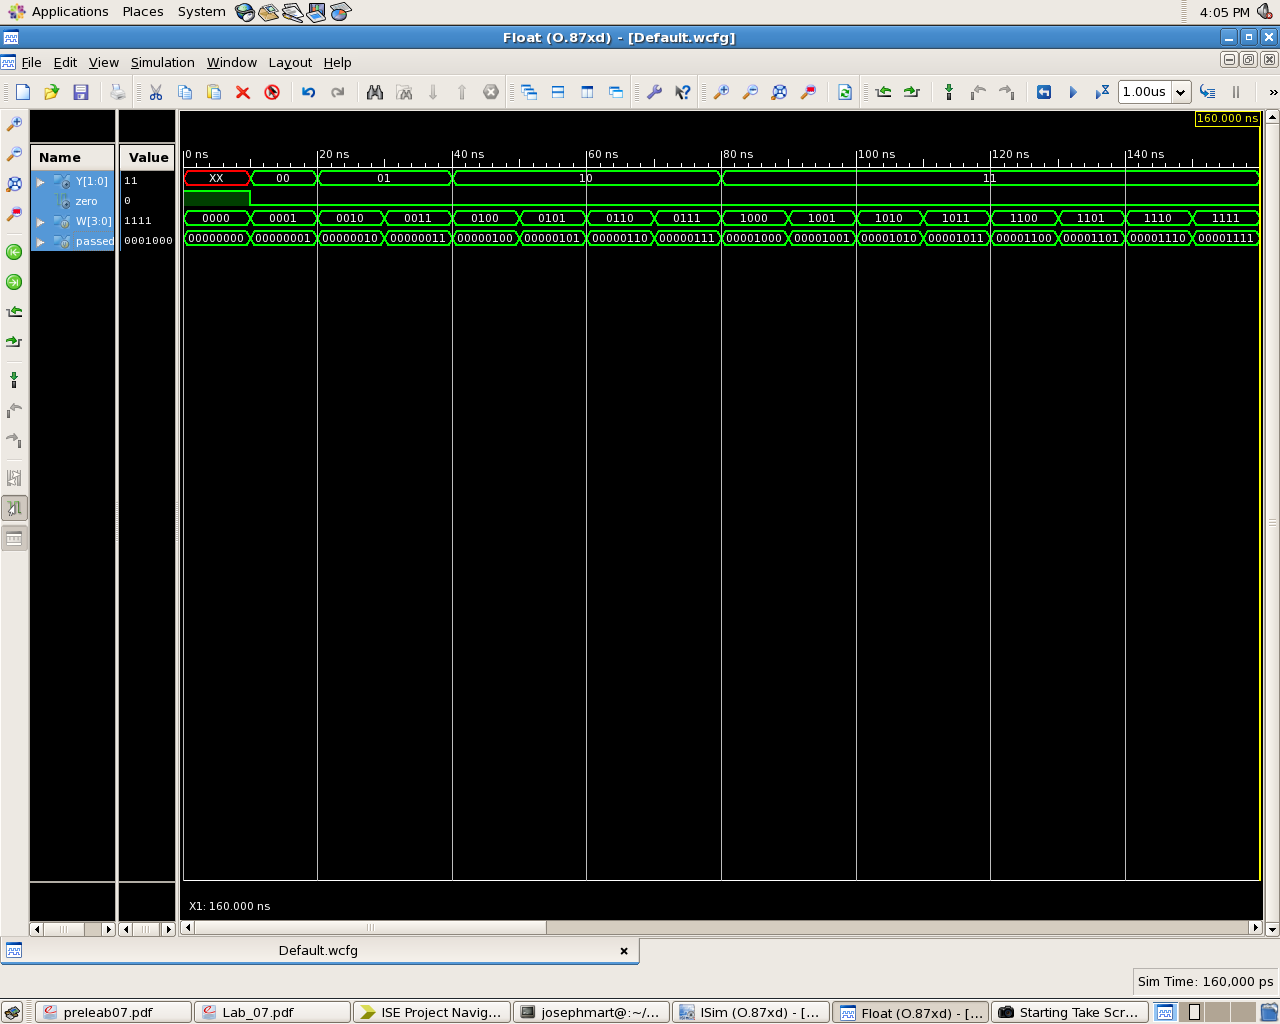
\includegraphics[scale=0.1]{2_3_2.png}
%     \caption{\textit{2-Bit 2:1 MUX Plots}}
%   \end{center}
% \end{figure}

\hspace{-15pt}\textbf{Experiment 3}


\section*{Conclutions}


\section*{Questions}

\begin{enumerate}
  \item \textbf{Include the source code with comments for all modules you simulated. You do not have to include test bench code. Code without comments will not be accepted!}

  \textit{In Report}

  \item \textbf{Include screenshots of all waveforms captured during simulation in addition to the test bench console output for each test bench simulation.}

  \textit{In Report}

  \item \textbf{Provide a comparison between behavioral Verilog used in this week’s lab and the structural and dataflow Verilog used in last week’s lab. What might be the advantages and disadvantages of each.}

  \item \textbf{Compare the process of bread-boarding digital circuit to implementing a digital circuit on an FPGA. State some advantages and disadvantages of each. Which process do you prefer?}
\end{enumerate}

\section*{Student Feedback}

\begin{enumerate}
  \item \textbf{What did you like most about the lab assignment and why? What did you like least aboub it and why?}
  \vspace{10pt}

  \item \textbf{Were there any section of the lab manual that were unclear? If so, what was unclear? Do you have any suggetions for improving the clarity?}
  \vspace{10pt}

  \item \textbf{What suggestions do you have to improve the overall lab assignment?}
  \vspace{10pt}

\end{enumerate}

\ifx
\begin{thebibliography}{1}
\bibitem{Verilog} Charles Kime \& Thomas Kaminski  \emph{Logic and Computer Design Fundamentals} \\ \hspace{15pt}\textit{http://www.cs.bilkent.edu.tr/~will/courses/CS223/Verilog/LCDF3_Verilog_Ch_4.pdf}
\end{thebibliography}

\section*{Attachments}
%Make sure to change these
Lab Notes, HelloWorld.ic, FooBar.ic
%\fi %comment me out

\begin{thebibliography}{9}
\bibitem{Verilog} Charles Kime & Thomas Kaminski  \emph{Logic and Computer Design Fundamentals} \textit{http://www.cs.bilkent.edu.tr/~will/courses/CS223/Verilog/LCDF3_Verilog_Ch_4.pdf}
\end{thebibliography}

%How to cite
Put your Problem statement here! Example of a Citation\cite[p.219]{Robotics}. Here's Another Citation\cite{Flueck}
\fi
\end{document}
